\documentclass[preview=true, border=10pt]{standalone}
%%%<
\usepackage{verbatim}
%%%>
\usepackage{tikz}
\usetikzlibrary{calc,positioning,shadows.blur,decorations.pathreplacing}
\usepackage{etoolbox}
\usepackage{siunitx}
\usepackage{nicefrac}

\definecolor{fillStrongForce}{HTML}{ffffff}
\definecolor{fillGluon}{HTML}{f6eff7}
\definecolor{fillQuarks}{HTML}{edf8fb}
\definecolor{fillEForce}{HTML}{f0f0f0}
\definecolor{fillPhoton}{HTML}{bdc9e1}
\definecolor{fillLeptons}{HTML}{b2e2e2}
\definecolor{fillWeakForce}{HTML}{d9d9d9}
\definecolor{fillWeakBosons}{HTML}{67a9cf}
\definecolor{fillNeutrinos}{HTML}{66c2a4}
\definecolor{fillSpinChargeFermions}{HTML}{e31a1c}

\newcommand{\SMTikzSize}{1.7}

\newcommand\particle[7][white]{%
  \begin{tikzpicture}[x=\SMTikzSize cm, y=\SMTikzSize cm]
    \path[fill=#1] (0.1*\SMTikzSize,0) -- (0.9,0)
        arc (90:0:0.1*\SMTikzSize cm) -- (1.0,-0.9) arc (0:-90:0.1*\SMTikzSize cm) -- (0.1,-1.0)
        arc (-90:-180:0.1*\SMTikzSize cm) -- (0,-0.1) arc(180:90:0.1*\SMTikzSize cm) -- cycle;
    \ifstrempty{#7}{}{\path[fill=gray!40!white]
        (0.55,-1) --(0.7,-1) -- (1.0,-0.7) -- (1.0,-0.55);}
    \ifstrempty{#6}{}{\path[fill=fillSpinChargeFermions] (0.7,0) -- (0.9,0)
        arc (90:0:0.1*\SMTikzSize cm) -- (1.0,-0.3);}
    \ifstrempty{#5}{}{\path[fill=fillSpinChargeFermions] (1.0,-0.7) -- (1.0,-0.9)
        arc (0:-90:0.1*\SMTikzSize cm) -- (0.7,-1.0);}
    \draw[\ifstrempty{#2}{dashed}{black}] (0.1,0) -- (0.9,0)
        arc (90:0:0.1*\SMTikzSize cm) -- (1.0,-0.9) arc (0:-90:0.1*\SMTikzSize cm) -- (0.1,-1.0)
        arc (-90:-180:0.1*\SMTikzSize cm) -- (0,-0.1) arc(180:90:0.1*\SMTikzSize cm) -- cycle;
    \ifstrempty{#7}{}{\node at(0.815,-0.815) [rotate=45,scale=0.4] {#7};}
    \ifstrempty{#6}{}{\node at(0.9,-0.1)  [nosep,scale=0.39] {#6};}
    \ifstrempty{#5}{}{\node at(0.91,-0.91)  [nosep,scale=0.41] {#5};}
    \ifstrempty{#4}{}{\node at(0.08,-0.2)  [nosep,anchor=west,scale=0.5]{#4};}
    \ifstrempty{#3}{}{\node at(0.1,-0.85) [nosep,anchor=west,scale=0.6] {#3};}
    \ifstrempty{#2}{}{\node at(0.1,-0.5)  [nosep,anchor=west,scale=1.5] {#2};}
  \end{tikzpicture}
}

\begin{document}
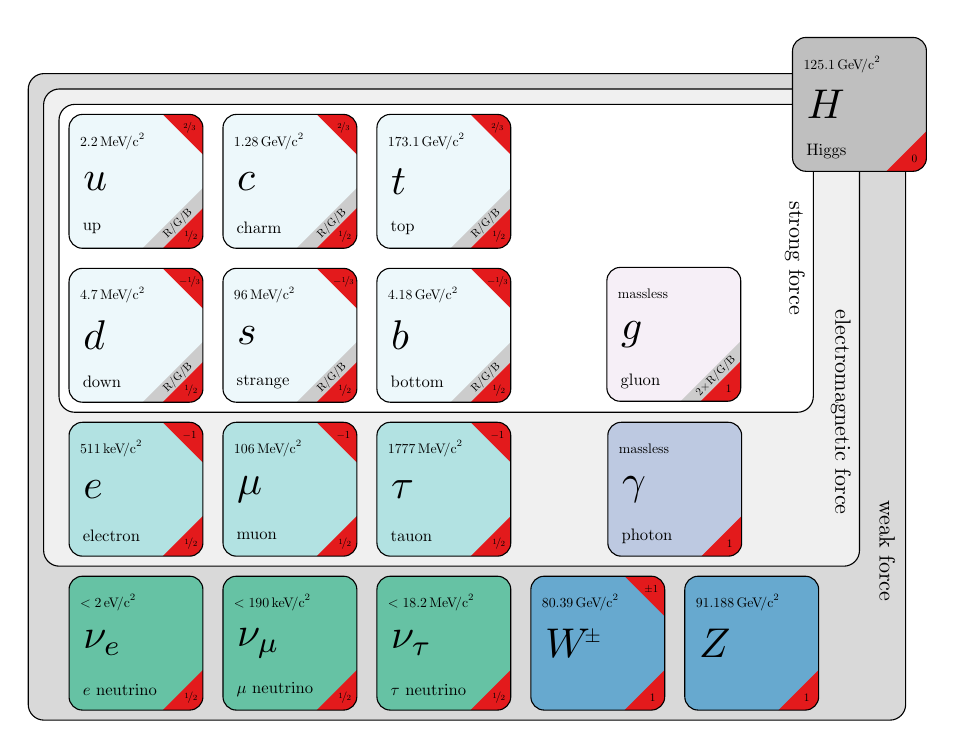
\begin{tikzpicture}[x=1.15*\SMTikzSize cm, y=1.15*\SMTikzSize cm,
                    round/.style = { rounded corners=2mm },
                    brace/.style = { decorate, decoration={brace, amplitude=5pt} },
                    mbrace/.style = { decorate, decoration={brace, amplitude=5pt, mirror} },
                    label/.style = { black, midway, scale=0.5, align=center },
                    toplabel/.style = { label, above=.5em, anchor=south },
                    leftlabel/.style = { label,rotate=-90,left=.5em,anchor=north },
                    bottomlabel/.style = { label, below=.5em, anchor=north },
                    force/.style = { rotate=-90,scale=0.8 },
                    legend/.style = { right,scale=0.4 },
                    nosep/.style = { inner sep=0pt },
                    generation/.style = { anchor=base }]
  \draw[round, fill=fillWeakForce] (-0.7,0.7) rectangle (5.0,-3.5);
  \draw[round, fill=fillEForce] (-0.6,0.6) rectangle (4.7,-2.5);
  \draw[round, fill=fillStrongForce] (-0.5,0.5) rectangle (4.4,-1.5);


  \node at(0, 0)   {\particle[fillQuarks]
                   {$u$}        {up}       {\SI{2.2}{\mathrm{Me\kern -0.1em V\!/}c^2}}{$\nicefrac{1}{2}$}{$\nicefrac{2}{3}$}{R/G/B}};
  \node at(0,-1)   {\particle[fillQuarks]
                   {$d$}        {down}    {\SI{4.7}{\mathrm{Me\kern -0.1em V\!/}c^2}}{$\nicefrac{1}{2}$}{$-\nicefrac{1}{3}$}{R/G/B}};
  \node at(0,-2)   {\particle[fillLeptons]
                   {$e$}        {electron}       {\SI{511}{\mathrm{ke\kern -0.1em V\!/}c^2}}{$\nicefrac{1}{2}$}{$-1$}{}};
  \node at(0,-3)   {\particle[fillNeutrinos]
                   {$\nu_e$}    {$e$ neutrino}         {$<\SI{2}{\mathrm{e\kern -0.1em V\!/}c^2}$}{$\nicefrac{1}{2}$}{}{}};
  \node at(1, 0)   {\particle[fillQuarks]
                   {$c$}        {charm}   {\SI{1.28}{\mathrm{Ge\kern -0.1em V\!/}c^2}}{$\nicefrac{1}{2}$}{$\nicefrac{2}{3}$}{R/G/B}};
  \node at(1,-1)   {\particle[fillQuarks]
                   {$s$}        {strange}  {\SI{96}{\mathrm{Me\kern -0.1em V\!/}c^2}}{$\nicefrac{1}{2}$}{$-\nicefrac{1}{3}$}{R/G/B}};
  \node at(1,-2)   {\particle[fillLeptons]
                   {$\mu$}      {muon}         {\SI{106}{\mathrm{Me\kern -0.1em V\!/}c^2}}{$\nicefrac{1}{2}$}{$-1$}{}};
  \node at(1,-3)   {\particle[fillNeutrinos]
                   {$\nu_\mu$}  {$\mu$ neutrino}    {$<\SI{190}{\mathrm{ke\kern -0.1em V\!/}c^2}$}{$\nicefrac{1}{2}$}{}{}};
  \node at(2, 0)   {\particle[fillQuarks]
                   {$t$}        {top}    {\SI{173.1}{\mathrm{Ge\kern -0.1em V\!/}c^2}}{$\nicefrac{1}{2}$}{$\nicefrac{2}{3}$}{R/G/B}};
  \node at(2,-1)   {\particle[fillQuarks]
                   {$b$}        {bottom}  {\SI{4.18}{\mathrm{Ge\kern -0.1em V\!/}c^2}}{$\nicefrac{1}{2}$}{$-\nicefrac{1}{3}$}{R/G/B}};
  \node at(2,-2)   {\particle[fillLeptons]
                   {$\tau$}     {tauon}          {\SI{1777}{\mathrm{Me\kern -0.1em V\!/}c^2}}{$\nicefrac{1}{2}$}{$-1$}{}};
  \node at(2,-3)   {\particle[fillNeutrinos]
                   {$\nu_\tau$} {$\tau$ neutrino}  {$<\SI{18.2}{\mathrm{Me\kern -0.1em V\!/}c^2}$}{$\nicefrac{1}{2}$}{}{}};
  \node at(3,-3)   {\particle[fillWeakBosons]
                   {$W^{\hspace{-.3ex}\scalebox{.5}{$\pm$}}$}
                                {}              {\SI{80.39}{\mathrm{Ge\kern -0.1em V\!/}c^2}}{1}{$\pm1$}{}};
  \node at(4,-3)   {\particle[fillWeakBosons]
                   {$Z$}        {}                    {\SI{91.188}{\mathrm{Ge\kern -0.1em V\!/}c^2}}{1}{}{}};
  \node at(3.5,-2) {\particle[fillPhoton]
                   {$\gamma$}   {photon}                        {massless}{1}{}{}};
  \node at(3.5,-1) {\particle[fillGluon]
                   {$g$}        {gluon}                    {massless}{1}{}{$2\!\times\!\mathrm{R/G/B}$}};
  \node at(4.7,0.5){\particle[gray!50!white]
                   {$H$}        {Higgs}              {\SI{125.1}{\mathrm{Ge\kern -0.1em V\!/}c^2}}{0}{}{}};

  \node at(4.28,-0.5) [force]      {strong force};
  \node at(4.58,-1.5) [force]    {electromagnetic force};
  \node at(4.88,-2.4) [force] {weak force};


  % \draw [brace] (-0.5,.8) -- (0.5,.8) node[toplabel]         {standard matter};
  % \draw [brace] (0.5,.8)  -- (2.5,.8) node[toplabel]         {unstable matter};
  % \draw [brace] (2.5,.8)  -- (4.5,.8) node[toplabel]          {force carriers};

  % \node at (0,1.2)   [generation] {1\tiny st};
  % \node at (1,1.2)   [generation] {2\tiny nd};
  % \node at (2,1.2)   [generation] {3\tiny rd};
  % \node at (2.8,1.2) [generation] {\tiny generation};
\end{tikzpicture}
\end{document}
